% !TeX program = xelatex
% !TeX encoding = UTF-8
% Sinh tu du lieu that trong code thuat toan/results/*.pt
\documentclass[11pt,a4paper]{article}

\usepackage{fontspec}
\usepackage{unicode-math}
\IfFontExistsTF{Times New Roman}{\setmainfont{Times New Roman}}{\setmainfont{Liberation Serif}}
\IfFontExistsTF{Cambria Math}{\setmathfont{Cambria Math}}{\setmathfont{LibertinusMath-Regular.otf}}

\usepackage[a4paper,top=2.2cm,bottom=2.2cm,left=2.2cm,right=2.0cm]{geometry}
\usepackage{graphicx}
\usepackage{booktabs}
\usepackage{tabularx}
\usepackage{array}
\usepackage{threeparttable}
\usepackage{makecell}
\usepackage{float}
\usepackage{caption}
\usepackage{xcolor}
\usepackage{enumitem}
\usepackage[hidelinks]{hyperref}

\definecolor{Accent}{HTML}{2E5A88}
\definecolor{Warn}{HTML}{9B4B4B}
\definecolor{BoxBg}{HTML}{F4F6F8}

\captionsetup{font=small,labelfont=bf,skip=5pt}
\renewcommand{\tablename}{Bảng}
\renewcommand{\figurename}{Hình}
\setlength{\parindent}{0pt}
\setlength{\parskip}{0.45em}
\newcolumntype{C}{>{\centering\arraybackslash}X}
\newcolumntype{R}{>{\raggedleft\arraybackslash}X}
\newcolumntype{L}{>{\raggedright\arraybackslash}X}
\newcommand{\best}[1]{\textbf{#1}}

\newcommand{\hopketqua}[1]{%
  \begin{center}\fcolorbox{Accent}{BoxBg}{\begin{minipage}{0.95\linewidth}
  \vspace{0.3em}#1\vspace{0.3em}
  \end{minipage}}\end{center}}

\title{\vspace{-1.2cm}\textbf{Báo cáo kết quả ước lượng và so sánh mô hình}\\[0.25em]
\large MS-GARCH-X Student-t cho hợp đồng tương lai VN30F1M}
\author{}
\date{}

\begin{document}
\maketitle
\vspace{-1.6cm}

\section*{Tóm tắt kết quả}
\hopketqua{
\textbf{Bốn kết luận chính.}
\begin{enumerate}[leftmargin=1.6em,itemsep=0.25em,topsep=0.3em]
  \item \textbf{Mô hình một chế độ thắng cả trong mẫu lẫn ngoài mẫu.} B3 (GARCH-X Student-t) đạt AIC thấp nhất (5648{,}87), BIC thấp nhất (5687{,}08) và QLIKE ngoài mẫu tốt nhất (0{,}9520), vượt M1 (MS-GARCH-X) ở cả ba tiêu chí dù M1 có log-hợp-lý cao hơn.
  \item \textbf{Variational Bayes cho dự báo mật độ tốt nhất với chi phí thấp.} M2 đạt điểm log âm nhỏ nhất (1{,}5354) trong 77{,}9 phút, so với 424{,}7 phút của M1.
  \item \textbf{MCMC thất bại.} Sau hai lần chạy được lưu, $\widehat{R}$ tốt nhất chỉ đạt 2{,}8379 (yêu cầu $<1{,}01$) và ESS nhỏ nhất 4{,}7; 71{,}06\% mẫu hậu nghiệm phải đổi nhãn trạng thái, tức danh tính trạng thái không ổn định ngay trong một lần chạy.
  \item \textbf{Cấu trúc chuyển trạng thái không được dữ liệu nhận dạng.} Bốn phương pháp cho $p_{11}$ trải từ 0{,}7329 đến 0{,}9986, tương ứng thời gian tồn tại trạng thái chênh nhau hai bậc độ lớn.
\end{enumerate}
}

\section{Danh mục mô hình và phương pháp}

\begin{table}[H]\centering
\caption{Các mô hình được ước lượng và phương pháp suy diễn tương ứng}
\begin{tabularx}{\textwidth}{l >{\raggedright\arraybackslash}p{3.1cm} C C C}
\toprule
\textbf{Mã} & \textbf{Đặc tả} & \textbf{Phân phối sai số} & \textbf{Số trạng thái} & \textbf{Phương pháp} \\
\midrule
B1 & GARCH(1,1) & Chuẩn & 1 & MLE \\
B2 & GARCH(1,1) & Student-t & 1 & MLE \\
B3 & GARCH-X & Student-t & 1 & MLE \\
B4 & MS-GARCH & Chuẩn & 2 & MLE \\
M1 & MS-GARCH-X & Student-t & 2 & MLE \\
M2 & MS-GARCH-X & Student-t & 2 & VB mean-field \\
M3 & MS-GARCH-X & Student-t & 2 & VB full-rank \\
M4 & MS-GARCH-X & Student-t & 2 & MCMC (NUTS) \\
R1 & MS-GARCH-X, $\nu_s$ riêng & Student-t & 2 & VB mean-field \\
\bottomrule
\end{tabularx}
\end{table}


\section{So sánh trong mẫu}

\begin{table}[H]\centering
\caption{Log-hợp-lý và tiêu chí thông tin (tập huấn luyện $1735$ quan sát)}
\begin{threeparttable}
\begin{tabularx}{\textwidth}{l C C C C C C}
\toprule
\textbf{Mô hình} & \textbf{Số tham số} & \textbf{Log-hợp-lý} & \textbf{AIC} & \textbf{Hạng AIC} & \textbf{BIC} & \textbf{Hạng BIC} \\
\midrule
B1 & 4 & -2944{,}90 & 5897{,}80 & 5 & 5919{,}63 & 5 \\
B2 & 5 & -2825{,}81 & 5661{,}62 & 3 & 5688{,}92 & 2 \\
B3 & 7 & -2817{,}43 & \best{5648{,}87} & 1 & \best{5687{,}08} & 1 \\
B4 & 10 & -2854{,}15 & 5728{,}29 & 4 & 5782{,}88 & 4 \\
M1 & 15 & -2810{,}29 & 5650{,}58 & 2 & 5732{,}46 & 3 \\
\bottomrule
\end{tabularx}
\begin{tablenotes}\small
\item Giá trị nhỏ hơn là tốt hơn ở cả AIC và BIC. M1 có log-hợp-lý cao nhất nhưng dùng $15$ tham số; sau khi phạt số tham số, B3 ($7$ tham số) vượt lên ở cả hai tiêu chí. Chênh lệch BIC giữa B3 và M1 là 45{,}38 điểm, tức bằng chứng mạnh nghiêng về mô hình một chế độ.
\end{tablenotes}
\end{threeparttable}
\end{table}

\begin{figure}[H]\centering
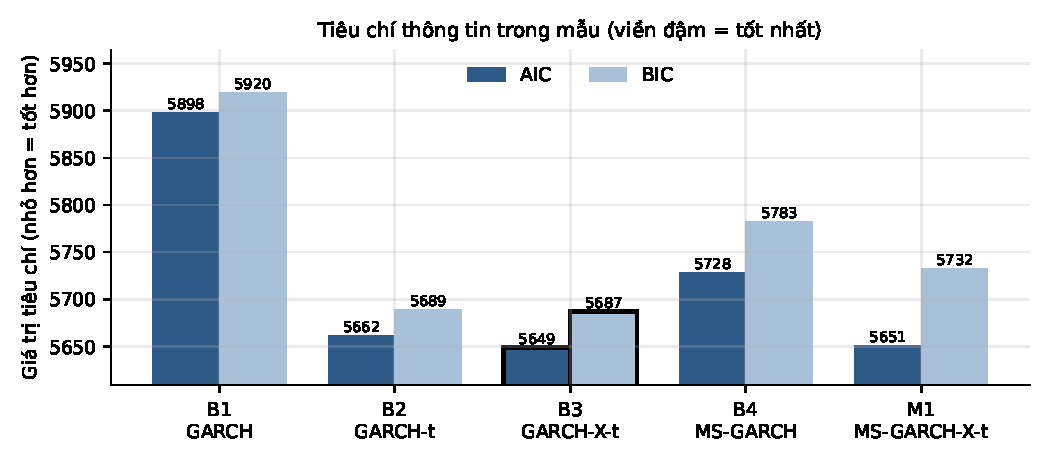
\includegraphics[width=\textwidth]{hinh_bao_cao/fig_ic.pdf}
\caption{Tiêu chí thông tin trong mẫu. Việc thêm biến ngoại sinh (B2 $\to$ B3) cải thiện mạnh hơn nhiều so với việc thêm cơ chế chuyển trạng thái (B3 $\to$ M1).}
\end{figure}


\section{So sánh ngoài mẫu}

\begin{table}[H]\centering
\caption{Dự báo biến động và mật độ ngoài mẫu ($435$ quan sát kiểm định)}
\begin{threeparttable}
\begin{tabularx}{\textwidth}{l C C C C C C}
\toprule
\textbf{Mô hình} & \textbf{MAE} & \textbf{RMSE} & \textbf{QLIKE} & \textbf{Hạng QLIKE} & \textbf{NLS} & \textbf{Hạng NLS} \\
\midrule
B1 & 1{,}2769 & 2{,}2799 & 0{,}9836 & 4 & 1{,}6812 & 8 \\
B2 & 1{,}3943 & 2{,}5233 & 0{,}9943 & 5 & 1{,}5455 & 6 \\
B3 & 1{,}1953 & 2{,}1654 & \best{0{,}9520} & 1 & 1{,}5385 & 4 \\
B4 & 1{,}3232 & 2{,}1970 & 1{,}0232 & 7 & 1{,}5736 & 7 \\
M1 & 1{,}3031 & 2{,}2625 & 0{,}9688 & 2 & 1{,}5373 & 2 \\
M2 & 1{,}2970 & 2{,}2259 & 0{,}9978 & 6 & \best{1{,}5354} & 1 \\
M3 & 1{,}9505 & 3{,}1874 & 1{,}1434 & 8 & 1{,}5392 & 5 \\
M4$^{*}$ & 1{,}3172 & 2{,}4334 & 0{,}9786 & 3 & 1{,}5383 & 3 \\
\bottomrule
\end{tabularx}
\begin{tablenotes}\small
\item Giá trị nhỏ hơn là tốt hơn ở mọi cột. QLIKE là tiêu chí chính cho dự báo phương sai; NLS (điểm log âm) là tiêu chí cho dự báo mật độ.
\item[$^{*}$] Số liệu M4 sinh từ mẫu hậu nghiệm \emph{chưa hội tụ} ($\widehat{R}=2{,}8379$). Báo cáo ở đây để đối chiếu, không dùng làm căn cứ kết luận.
\end{tablenotes}
\end{threeparttable}
\end{table}

\begin{figure}[H]\centering
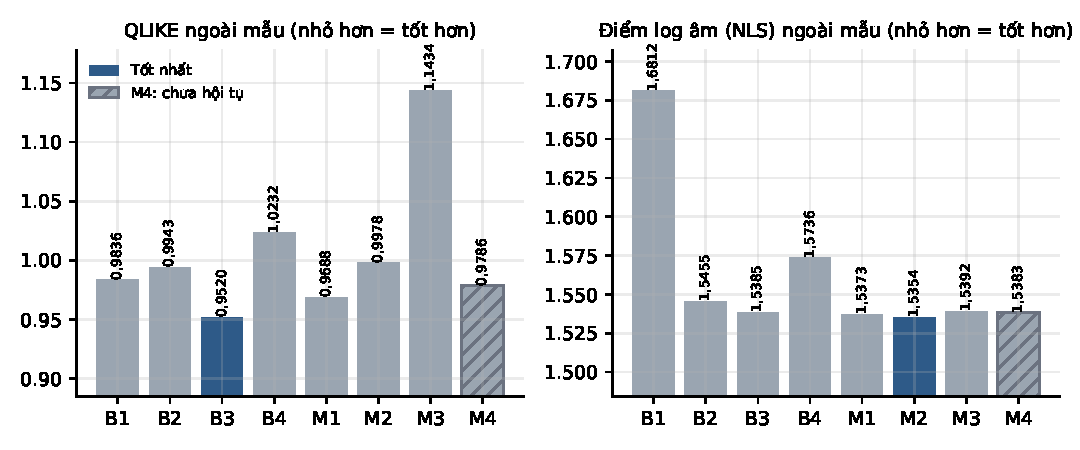
\includegraphics[width=\textwidth]{hinh_bao_cao/fig_oos.pdf}
\caption{Hai tiêu chí ngoài mẫu xếp hạng khác nhau: QLIKE ưu tiên B3, còn điểm log ưu tiên M2. Điều này phản ánh QLIKE đo dự báo phương sai điểm, còn điểm log đo toàn bộ hình dạng phân phối, nơi bất định tham số của phương pháp Bayes có giá trị.}
\end{figure}


\section{Kiểm định giá trị chịu rủi ro (VaR)}

\begin{table}[H]\centering
\caption{Kiểm định VaR ngoài mẫu ở hai mức tin cậy}
\begin{threeparttable}
\begin{tabularx}{\textwidth}{l C C C C C C}
\toprule
& \multicolumn{3}{c}{\textbf{Mức $\alpha=1\%$} (kỳ vọng $4{,}35$)} & \multicolumn{3}{c}{\textbf{Mức $\alpha=5\%$} (kỳ vọng $21{,}75$)} \\
\cmidrule(lr){2-4}\cmidrule(lr){5-7}
\textbf{Mô hình} & \makecell{\textbf{Số}\\\textbf{vi phạm}} & \makecell{\textbf{Kupiec}\\$p$} & \makecell{\textbf{Christ.}\\$p_{cc}$} & \makecell{\textbf{Số}\\\textbf{vi phạm}} & \makecell{\textbf{Kupiec}\\$p$} & \makecell{\textbf{Christ.}\\$p_{cc}$} \\
\midrule
B1 & 10 & \textcolor{Warn}{0{,}020} & 0{,}052 & 19 & 0{,}537 & 0{,}425 \\
B2 & 5 & 0{,}760 & 0{,}900 & 25 & 0{,}484 & 0{,}701 \\
B3 & 5 & 0{,}760 & 0{,}900 & 26 & 0{,}364 & 0{,}358 \\
B4 & 4 & 0{,}864 & 0{,}949 & 25 & 0{,}484 & 0{,}701 \\
M1 & 5 & 0{,}760 & 0{,}900 & 28 & 0{,}187 & 0{,}285 \\
M2 & 4 & 0{,}864 & 0{,}949 & 29 & 0{,}128 & 0{,}115 \\
M3 & 4 & 0{,}864 & 0{,}949 & 26 & 0{,}364 & 0{,}358 \\
M4$^{*}$ & 4 & 0{,}864 & 0{,}949 & 25 & 0{,}484 & 0{,}370 \\
\bottomrule
\end{tabularx}
\begin{tablenotes}\small
\item $p$ nhỏ hơn $0{,}05$ (in màu đỏ) nghĩa là bác bỏ mô hình. Chỉ B1 --- mô hình giả định phân phối chuẩn --- bị Kupiec bác bỏ ở mức $1\%$ với $10$ vi phạm; mọi mô hình Student-t đều vượt qua cả hai kiểm định ở cả hai mức. Đây là bằng chứng trực tiếp cho vai trò của đuôi dày trong quản trị rủi ro.
\item[$^{*}$] Xem chú thích về M4 ở Bảng 3.
\end{tablenotes}
\end{threeparttable}
\end{table}

\begin{figure}[H]\centering
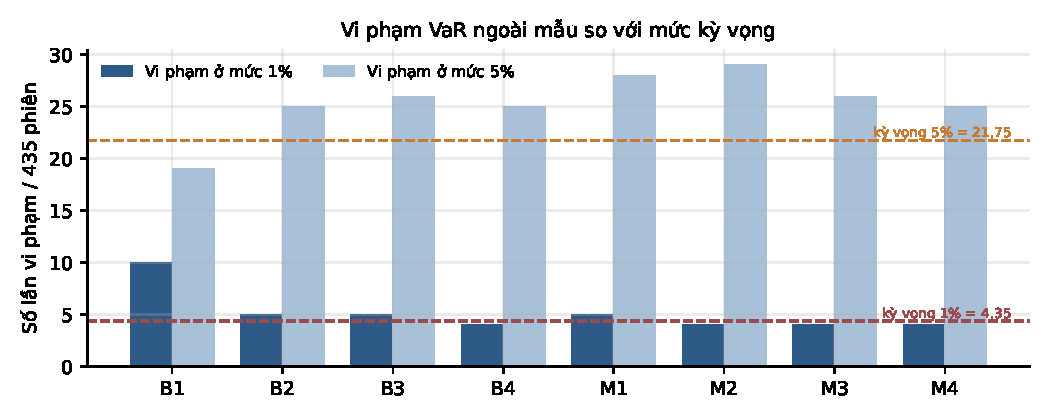
\includegraphics[width=\textwidth]{hinh_bao_cao/fig_var.pdf}
\caption{Số lần vi phạm VaR so với mức kỳ vọng lý thuyết (đường đứt nét). B1 vượt xa mức kỳ vọng ở ngưỡng $1\%$; các mô hình Student-t đều bám sát.}
\end{figure}


\section{So sánh bốn phương pháp ước lượng trên cùng một mô hình}

Mục này trả lời câu hỏi trung tâm: bốn phương pháp suy diễn cho kết quả \emph{khác nhau đến mức nào} khi áp dụng cho cùng một đặc tả MS-GARCH-X Student-t và cùng một tập dữ liệu.

\begin{table}[H]\centering
\caption{Ước lượng điểm và khoảng $95\%$ của các tham số then chốt}
\begin{threeparttable}
\begin{tabularx}{\textwidth}{l C C C C}
\toprule
\textbf{Tham số} & \textbf{MLE (M1)} & \textbf{VB mean-field (M2)} & \textbf{VB full-rank (M3)} & \textbf{MCMC (M4)$^{*}$} \\
\midrule
$\alpha_1$ & \makecell{0{,}1091\\\scriptsize[0{,}056; 0{,}162]} & \makecell{0{,}2709\\\scriptsize[0{,}104; 0{,}485]} & \makecell{0{,}2721\\\scriptsize[0{,}070; 0{,}472]} & \makecell{0{,}2077\\\scriptsize[0{,}061; 0{,}428]} \\
$\alpha_2$ & \makecell{0{,}3288\\\scriptsize[0{,}048; 0{,}610]} & \makecell{0{,}2312\\\scriptsize[0{,}156; 0{,}551]} & \makecell{0{,}3823\\\scriptsize[0{,}123; 0{,}666]} & \makecell{0{,}4056\\\scriptsize[0{,}181; 0{,}647]} \\
$\beta_1$ & \makecell{0{,}8463\\\scriptsize[0{,}773; 0{,}920]} & \makecell{0{,}2985\\\scriptsize[0{,}157; 0{,}648]} & \makecell{0{,}5980\\\scriptsize[0{,}424; 0{,}816]} & \makecell{0{,}4594\\\scriptsize[0{,}212; 0{,}688]} \\
$\beta_2$ & \makecell{0{,}3006\\\scriptsize[-0{,}155; 0{,}756]} & \makecell{0{,}6268\\\scriptsize[0{,}284; 0{,}688]} & \makecell{0{,}6468\\\scriptsize[0{,}466; 0{,}838]} & \makecell{0{,}6423\\\scriptsize[0{,}232; 0{,}836]} \\
$p_{11}$ & \makecell{0{,}9986\\\scriptsize[0{,}996; 1{,}001]} & \makecell{0{,}7329\\\scriptsize[0{,}558; 0{,}945]} & \makecell{0{,}8675\\\scriptsize[0{,}667; 0{,}957]} & \makecell{0{,}8239\\\scriptsize[0{,}651; 0{,}964]} \\
$p_{22}$ & \makecell{0{,}9932\\\scriptsize[0{,}982; 1{,}004]} & \makecell{0{,}9199\\\scriptsize[0{,}703; 0{,}966]} & \makecell{0{,}8441\\\scriptsize[0{,}659; 0{,}953]} & \makecell{0{,}7614\\\scriptsize[0{,}629; 0{,}891]} \\
$\nu$ & \makecell{4{,}0761\\\scriptsize[3{,}237; 4{,}915]} & \makecell{3{,}5204\\\scriptsize[3{,}200; 3{,}905]} & \makecell{2{,}9779\\\scriptsize[2{,}656; 3{,}435]} & \makecell{4{,}0741\\\scriptsize[3{,}414; 5{,}025]} \\
\bottomrule
\end{tabularx}
\begin{tablenotes}\small
\item Với MLE, khoảng là $\hat\theta\pm1{,}96\,\mathrm{SE}$ (delta method từ Hessian quan sát); với ba phương pháp Bayes, khoảng là phân vị $2{,}5\%$ và $97{,}5\%$ của hậu nghiệm. Mẫu hậu nghiệm của cả ba đã được sắp xếp lại nhãn trạng thái theo quy ước ``trạng thái 1 là trạng thái biến động thấp'' trước khi tính.
\item Khoảng của $p_{11}$ và $p_{22}$ theo MLE vượt quá $1$ --- dấu hiệu nghiệm nằm sát biên không gian tham số, khiến xấp xỉ tiệm cận chuẩn không còn hợp lệ.
\item[$^{*}$] Xem chú thích về M4 ở Bảng 3.
\end{tablenotes}
\end{threeparttable}
\end{table}

\begin{figure}[H]\centering
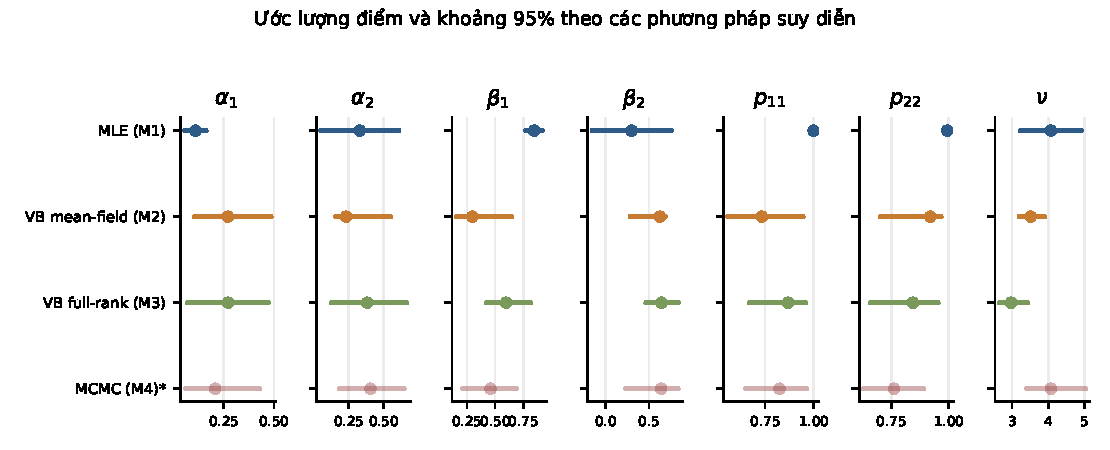
\includegraphics[width=\textwidth]{hinh_bao_cao/fig_forest.pdf}
\caption{Bốn phương pháp đồng thuận cao ở $\nu$ và $\alpha_2$, nhưng phân kỳ mạnh ở $\beta_1$ và đặc biệt ở $p_{11}$, $p_{22}$ --- đúng những tham số điều khiển cấu trúc chuyển trạng thái.}
\end{figure}


\begin{table}[H]\centering
\caption{Hệ quả kinh tế: thời gian tồn tại kỳ vọng của mỗi trạng thái}
\begin{threeparttable}
\begin{tabularx}{\textwidth}{l C C C}
\toprule
\textbf{Đại lượng} & \textbf{MLE (M1)} & \textbf{VB mean-field (M2)} & \textbf{MCMC (M4)$^{*}$} \\
\midrule
$d_1$ (trạng thái biến động thấp) & 717{,}9 phiên & 3{,}7 phiên & 5{,}7 phiên \\
$d_2$ (trạng thái biến động cao) & 147{,}0 phiên & 12{,}5 phiên & 4{,}2 phiên \\
\bottomrule
\end{tabularx}
\begin{tablenotes}\small
\item $d_s = 1/(1-p_{ss})$. Ba phương pháp cho ba câu trả lời chênh nhau tới hai bậc độ lớn trên cùng một bộ dữ liệu: MLE mô tả các chế độ kéo dài nhiều năm, còn VB và MCMC mô tả các chế độ chỉ vài phiên đến vài tuần. Đây là biểu hiện rõ nhất của việc cấu trúc chuyển trạng thái không được nhận dạng từ dữ liệu.
\item[$^{*}$] Xem chú thích về M4 ở Bảng 3.
\end{tablenotes}
\end{threeparttable}
\end{table}


\section{Chẩn đoán hội tụ}

\begin{table}[H]\centering
\caption{Chẩn đoán hội tụ MCMC (NUTS), bốn chuỗi $\times$ $400$ mẫu}
\begin{threeparttable}
\begin{tabularx}{\textwidth}{l C C C C}
\toprule
& \multicolumn{2}{c}{\textbf{Lần 1}: ma trận đường chéo, warmup $250$} & \multicolumn{2}{c}{\textbf{Lần 2}: ma trận đặc, warmup $1000$} \\
\cmidrule(lr){2-3}\cmidrule(lr){4-5}
\textbf{Tham số} & $\widehat{R}$ & ESS & $\widehat{R}$ & ESS \\
\midrule
$\mu$ & 3{,}3433 & 4{,}5 & 2{,}2512 & 5{,}1 \\
$\omega$ & 3{,}3918 & 4{,}5 & 2{,}6420 & 4{,}8 \\
$\alpha$ & 3{,}7634 & 4{,}4 & 2{,}4097 & 5{,}0 \\
$\beta$ & 3{,}5078 & 4{,}5 & 2{,}8379 & 4{,}7 \\
$\gamma$ & 3{,}3459 & 4{,}5 & 2{,}4622 & 4{,}9 \\
$p_{11}$ & 4{,}0601 & 4{,}4 & 1{,}9572 & 5{,}6 \\
$p_{22}$ & 3{,}4267 & 4{,}5 & 2{,}2444 & 5{,}1 \\
$\nu$ & 3{,}7612 & 4{,}4 & 1{,}4276 & 8{,}5 \\
\midrule
\textbf{Xấu nhất} & \textcolor{Warn}{4{,}0601} & 4{,}4 & \textcolor{Warn}{2{,}8379} & 4{,}7 \\
Số lần phân kỳ & \multicolumn{2}{c}{14} & \multicolumn{2}{c}{13} \\
\bottomrule
\end{tabularx}
\begin{tablenotes}\small
\item Tiêu chuẩn chấp nhận là $\widehat{R}<1{,}01$ và ESS đủ lớn (thông thường $>400$). Tăng warmup gấp bốn lần và chuyển sang ma trận khối lượng đặc chỉ kéo $\widehat{R}$ từ 4{,}06 xuống 2{,}84 --- vẫn cách rất xa ngưỡng. ESS quanh $5$ trên $1600$ mẫu nghĩa là bốn chuỗi gần như đứng yên tại bốn vị trí khác nhau.
\end{tablenotes}
\end{threeparttable}
\end{table}

\begin{table}[H]\centering
\caption{Tỷ lệ mẫu hậu nghiệm phải đổi nhãn trạng thái}
\begin{tabularx}{\textwidth}{l C C}
\toprule
\textbf{Mô hình} & \textbf{Tỷ lệ đổi nhãn} & \textbf{Diễn giải} \\
\midrule
M2: VB mean-field & 6{,}60\% & Ổn định: hầu hết mẫu đã đúng quy ước \\
M3: VB full-rank & 63{,}80\% & Bất ổn: gần một phép hoán vị toàn cục \\
M4: MCMC & 71{,}06\% & Bất ổn nặng: gần mức ngẫu nhiên $50\%$ \\
R1: VB, $\nu_s$ riêng & 91{,}70\% & Bất ổn: chủ yếu là hoán vị toàn cục \\
\bottomrule
\end{tabularx}
\end{table}

\begin{figure}[H]\centering
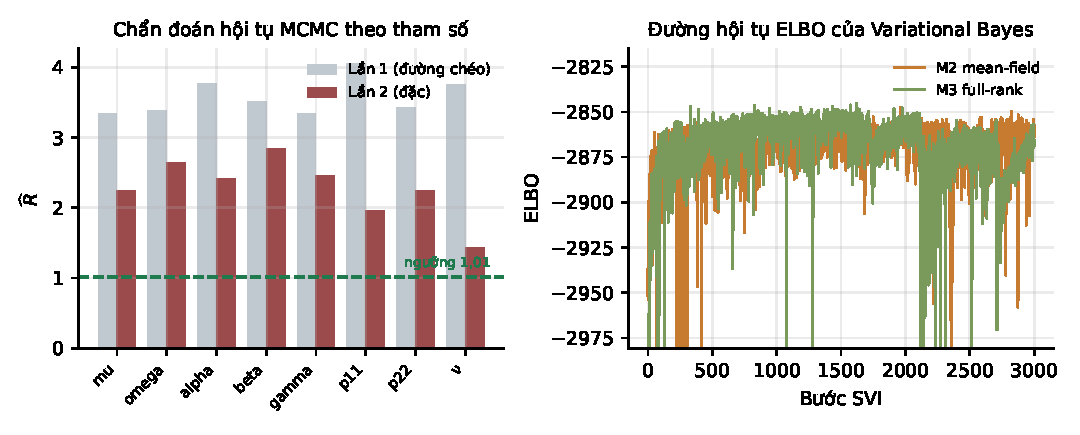
\includegraphics[width=\textwidth]{hinh_bao_cao/fig_conv.pdf}
\caption{Trái: $\widehat{R}$ theo tham số ở hai lần chạy MCMC, không lần nào chạm ngưỡng $1{,}01$. Phải: ELBO của hai biến thể Variational Bayes dao động quanh một mức ổn định sau khoảng một nghìn bước, cho thấy vấn đề hội tụ là đặc thù của MCMC chứ không phải của bài toán tối ưu nói chung.}
\end{figure}


\section{Chi phí tính toán}

\begin{table}[H]\centering
\caption{Thời gian ước lượng theo mô hình}
\begin{threeparttable}
\begin{tabularx}{\textwidth}{l C C C}
\toprule
\textbf{Mô hình} & \textbf{Phương pháp} & \textbf{Thời gian (phút)} & \textbf{Kết quả dùng được?} \\
\midrule
B1 & MLE & 13{,}6 & Có \\
B2 & MLE & 13{,}7 & Có \\
B3 & MLE & 14{,}6 & Có \\
B4 & MLE & 157{,}4 & Có \\
M1 & MLE & 424{,}7 & Có \\
M2 & VB mean-field & 77{,}9 & Có \\
M3 & VB full-rank & 77{,}2 & Có \\
R1 & VB mean-field & 76{,}2 & Có \\
M4 & MCMC (NUTS) & 3840{,}0 & \textcolor{Warn}{\textbf{Không}} \\
\bottomrule
\end{tabularx}
\begin{tablenotes}\small
\item Thời gian M4 là tổng cộng dồn của các lần chạy trên bốn tiến trình song song. Kết luận về đánh đổi chi phí rất rõ: phương pháp đắt nhất không cho kết quả dùng được, còn phương pháp rẻ hơn năm lần so với MLE (VB mean-field) lại cho dự báo mật độ tốt nhất.
\end{tablenotes}
\end{threeparttable}
\end{table}

\begin{figure}[H]\centering
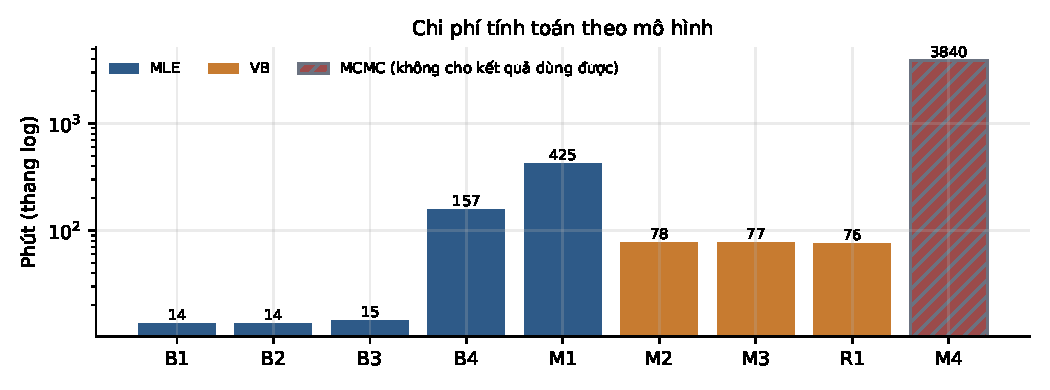
\includegraphics[width=\textwidth]{hinh_bao_cao/fig_cost.pdf}
\caption{Chi phí tính toán trên thang logarit. Khoảng cách giữa mô hình một chế độ và hai chế độ là hơn một bậc độ lớn.}
\end{figure}


\section{Nghiên cứu mô phỏng}

Trên dữ liệu thật không biết tham số đúng, nên chất lượng ước lượng được đánh giá bổ sung bằng mô phỏng tám kịch bản $S_1$--$S_8$ với tham số đã biết trước.

\begin{table}[H]\centering
\caption{Kết quả mô phỏng gộp trên tám kịch bản}
\begin{threeparttable}
\begin{tabularx}{\textwidth}{l C C C C C}
\toprule
\textbf{Phương pháp} & \textbf{Số lần lặp} & \textbf{$|$Độ chệch$|$ TB} & \textbf{RMSE TB} & \textbf{Coverage $95\%$} & \textbf{Brier} \\
\midrule
MLE & 225 & 0{,}2965 & 0{,}4983 & -- & 0{,}5307 \\
VB mean-field & 120 & 0{,}5347 & 0{,}5784 & 0{,}331 & 0{,}5811 \\
MCMC & 3 & 0{,}6224 & 0{,}6427 & 0{,}511 & 0{,}5406 \\
\bottomrule
\end{tabularx}
\begin{tablenotes}\small
\item Độ chệch và RMSE lấy trung bình trên các tham số có thang đo khác nhau, nên chỉ dùng để so sánh thô giữa các phương pháp. Coverage lý tưởng là $0{,}95$; cả hai phương pháp Bayes đều thấp hơn nhiều, tức khoảng tin cậy hậu nghiệm \emph{hẹp hơn thực tế} --- chúng đánh giá thấp mức bất định. MLE không sinh khoảng tin cậy trong quy trình mô phỏng nên không tính được coverage.
\item Số lần lặp của MCMC rất nhỏ ($3$) do chi phí tính toán, nên các con số ở hàng này chỉ mang tính tham khảo.
\end{tablenotes}
\end{threeparttable}
\end{table}

\begin{figure}[H]\centering
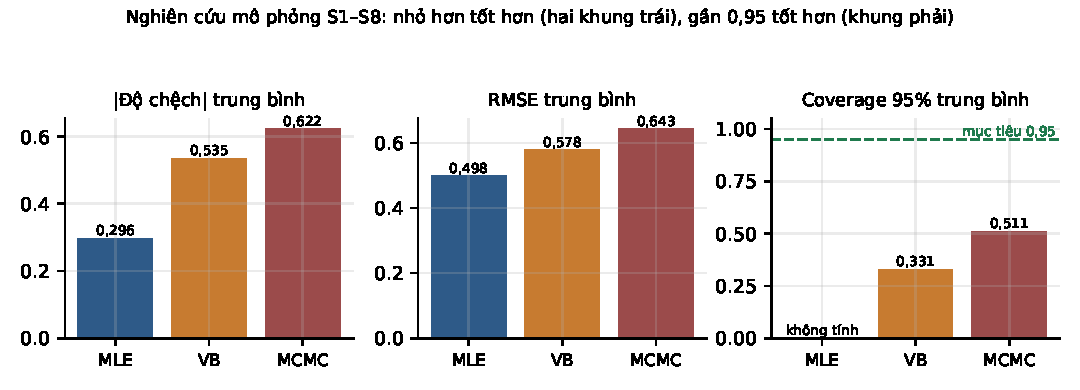
\includegraphics[width=\textwidth]{hinh_bao_cao/fig_sim.pdf}
\caption{MLE khôi phục tham số chính xác nhất trên dữ liệu mô phỏng; cả hai phương pháp Bayes đều đánh giá thấp bất định một cách đáng kể.}
\end{figure}


\section{Kết luận so sánh}

\begin{table}[H]\centering
\caption{Nên dùng phương pháp nào cho mục đích nào}
\begin{threeparttable}
\begin{tabularx}{\textwidth}{L C L}
\toprule
\textbf{Mục đích} & \textbf{Lựa chọn} & \textbf{Căn cứ} \\
\midrule
Dự báo phương sai điểm & B3 (GARCH-X, MLE) & QLIKE 0{,}9520 --- tốt nhất; đồng thời AIC và BIC thấp nhất \\
Dự báo mật độ / VaR & M2 (VB mean-field) & NLS 1{,}5354 --- tốt nhất; vượt qua mọi kiểm định VaR \\
Ước lượng tham số có sai số chuẩn & B3 (MLE) & Hội tụ ở mọi điểm khởi tạo, nghiệm không sát biên \\
Suy diễn Bayes đầy đủ cho MS-GARCH-X & \textcolor{Warn}{Chưa khả thi} & MCMC không hội tụ; VB đánh giá thấp bất định \\
\bottomrule
\end{tabularx}
\begin{tablenotes}\small
\item Kết luận bao trùm: trên dữ liệu VN30F1M hiện có, việc bổ sung \emph{biến ngoại sinh} mang lại cải thiện rõ rệt và ổn định, trong khi việc bổ sung \emph{cơ chế chuyển trạng thái ẩn} làm tăng đáng kể chi phí tính toán và độ bất định của kết luận mà không cải thiện dự báo ngoài mẫu.
\end{tablenotes}
\end{threeparttable}
\end{table}

\vfill
\begin{center}\small\textcolor{gray}{%
Toàn bộ số liệu trong báo cáo này được trích xuất trực tiếp từ
\texttt{code thuật toán/results/*.pt} và không nhập tay.}
\end{center}

\end{document}
